\documentclass{article}
\usepackage[utf8]{inputenc}
\usepackage[spanish]{babel}
\usepackage{amsmath, amsfonts, amsthm, amssymb, mathtools}
\usepackage{hyperref, url}
\usepackage[dvipsnames]{xcolor}
\usepackage{fancyhdr}
\usepackage[margin=2.54cm]{geometry}
\usepackage{graphicx, subcaption}
\usepackage{tabularx, ragged2e, booktabs}
\usepackage{float}
\usepackage[spanish]{cleveref}

\usepackage{tikz}
\usetikzlibrary{patterns}
\usepackage{scalerel}
\usepackage{pict2e}
\usepackage{tkz-euclide}
\usetikzlibrary{arrows.meta}
\usetikzlibrary{shadows}
\usetikzlibrary{external}
\usetikzlibrary{decorations.pathmorphing}
\usetikzlibrary{shapes.geometric}
\usetikzlibrary{snakes}
\usepackage{pgfplots}
\pgfplotsset{compat=newest}
\usepgfplotslibrary{statistics}
\usepgfplotslibrary{fillbetween}

\hypersetup{
	colorlinks=true,
	linkcolor=black,
	urlcolor=blue,
	pdftitle={2024-04-20 - Documento Protocolario 06 - Mittle-Seminar},
	pdfauthor={Julian Avila}
}
\urlstyle{same}

\theoremstyle{definition}
\newtheorem*{definition}{Definición}

\title{\textbf{Documento Protocolario 06}\\ \small{Mittle-Seminar}}
\date{\today}

\pagestyle{fancy}
\fancyhead{}
\fancyfoot{}
\lhead{Protocolo 06}
\rhead{Mittle-Seminar}

\begin{document}
\maketitle
\thispagestyle{fancy}
\hrule

\section{Reprogramación}
Siendo aproximadamente las 8:40 del 20 de Abril, 2024, se propone una reprogramación de futuros temas de exposición y fechas las para secciones del seminario. Se designa a Julian Avila como el responsable de llevar el protocolo de la sección.

\begin{itemize}
	\item Corchetes de Poisson (Zaudi Goméz, Julián Aros) - 25 de Abril
	\item Teorema de Noether (Mauricio Guevara) - 4 de Mayo
	\item Transformaciones canónicas (Camilo Huertas) - 11 de Mayo
	\item Dispersión de Rutherford (Sebastian Rodriguez, Issabela Ortiz) - 13 de Mayo
	\item Ensambles (Nicolas Sandoval, Daniela Torres) - 13 de Mayo
	\item Gases Versión 1. (Julian Avila) - 25 de Mayo
	\item Gases Versión 2. (Andres Torres) - 25 de Mayo
	\item Potenciales Termodinámicos (Alexei Duran, Diego Acosta) - 1 de Junio
\end{itemize}

%TODO Add memebrs

\section{Inicio de Sección y Plano Inclinado}
A las 9:07, comienza la exposición a cargo de Sebastián Manrique y Santiago Talero, titulada \textbf{El Plano Inclinado y la Maquina de Atwood Simple}.

Se utilizan dos sistemas comunes en física para explicar el concepto de ligadura o constricción.

El sistema consiste en una masa $m$ sobre un plano inclinado un angulo $\alpha$, sin fricción, como se muestra en la \Cref{fig:inclained_plane}.

\begin{figure}[H]
	\centering
	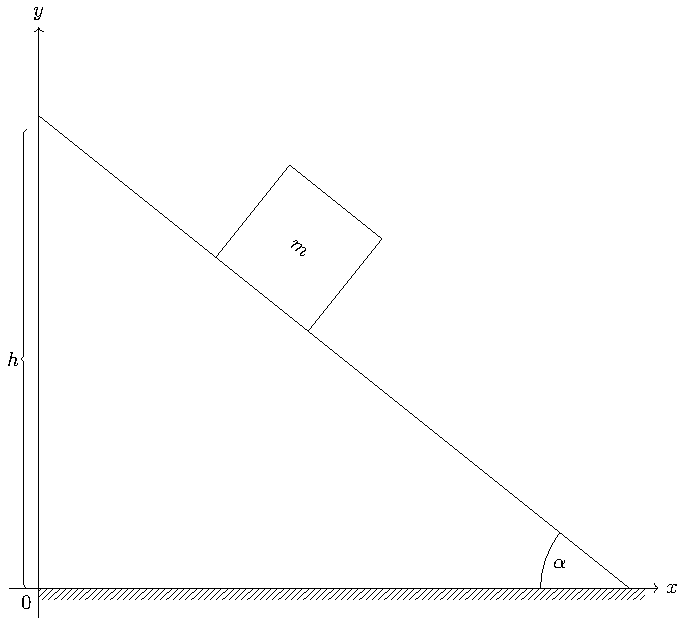
\includegraphics[width=0.30\textwidth]{./Images/inclined-plane.pdf}
	\caption{Diagrama del Plano Inclinado}
	\label{fig:inclained_plane}
\end{figure}

Como una primera definición simple de ligadura se dice que: Es una restricción que se le impone al sistema.

Para el plano inclinado se tienen las siguientes condiciones:
\begin{equation}
	\begin{cases}
		z = 0 &\implies f_1^{(h)} = 0 \\
		y = -x\tan{\alpha} + h &\implies f_2^{(h)} = y + x\tan{\alpha} - h = 0
	\end{cases}
\end{equation}

Estas ligaduras con de tipo holónoma esclerónoma. Al ser holónomas, se denotan por $f^{(h)}$, y ambas surgen de la construcción del sistema. Al no presentar movimiento en la coordenada $z$, esta se considera como $0$, mientras que $y$ solo puede variar en la linea recta dada por la inclinación del plano.

Después de identificar las ligaduras del sistema, se determina el numero mínimo de coordenadas generalizadas necesarias para describir el sistema utilizando la siguiente fórmula:

\begin{gather}
	s = 3N - K^{(h)} \label{eq:minim_coordinates}\\
	s = 3(1) - 2 \\
	\therefore s = 1
\end{gather}

donde $N$ es el numero de cuerpos del sistema y $K^{(h)}$ el numero de ligaduras del sistema, resultando en un mínimo de 1 coordenada generalizada para este caso especifico.

La energía cinética y la energía potencial del sistema estarían dadas por:

\begin{align}
	T &= \frac{1}{2} m \left(\dot{x}^2 + (-\dot{x}\tan{\alpha})^2 \right) \\
	V &= mg\left(x\tan{\alpha} + h \right)
\end{align}

El lagrangiano es entonces:

\begin{equation}
	\mathcal{L} = \frac{1}{2}m\dot{x}\sec^2{\alpha} + mgx\tan{\alpha} - mgh
\end{equation}

en términos de solo una coordenada.

\subsection{Preguntas emergentes y aclaraciones}
\emph{¿Cuál es la diferencia entre los tipos de ligadura holónomas y no holónomas?}
\begin{itemize}
	\item Las ligaduras holónomas se pueden representar por una igualdad i.e. $f(r_i, t) = 0$, mientras que las no holónomas se representan por una desigualdad e.g. $f(r_i, t) < 0$
\end{itemize}

	El director Alfonso Leyva pregunta: \emph{¿Cuántos son los grados de libertad del sistema?} Es un 1 grado de libertad, siendo la coordenada $x$ el eje de movimiento. El director realiza otra pregunta, \emph{Si está en el plano $xy$, ¿por qué no se toma $y$?} La razón es que $y$ depende de $x$, es decir, el movimiento está parametrizado con dependencia en $x$, resultando en un solo grado de libertad.

\subsection{Ecuación de movimiento del sistema}
Retomando con la exposición, al tener el Lagrangiano del sistema dependiente de una solo coordenada, se obtiene la ecuación de movimiento usando la ecuación de Euler-Lagrange:

\begin{gather}
	m\ddot{x}\sec^2{\alpha} - mg\tan{\alpha} = 0 \\
	\therefore \ddot{x} = g\sin{\alpha}\cos{\alpha}
\end{gather}

A partir de esta ultima ecuación se puede obtener la expresión para la velocidad y posición por mediante integración

\begin{align}
	\dot{x} &= gt\sin{\alpha}\cos{\alpha} + A \\
	x       &= \frac{1}{2} gt^{2} \sin{\alpha}\cos{\alpha} + At + B
\end{align}

Donde $A$ y $B$ son constantes que se determinan utilizando las condiciones iniciales del sistema.

\section{Maquina de Atwood Simple}
La maquina de Atwood simple consiste de dos masas conectadas por una cuerda la cual reposa sobre una polea. Es simple debido a que se toma la cuerda como inextensible y sin masa, al igual que la polea. La polea no presenta fricción con la cuerda y se presenta el diagrama en la \Cref{fig:atwood_machine}. La maquina cuenta con dos propiedades que la define:

\begin{itemize}
	\item Si $m_1 = m_2 \implies a = 0$ i.e. si las masas son iguales no se presentara aceleración.
	\item Si $m_1 \ne m_2 \implies a \ne 0$ i.e. si las masas son diferentes el movimiento sera acelerado.
\end{itemize}


\begin{figure}[htbp!]
	\centering
	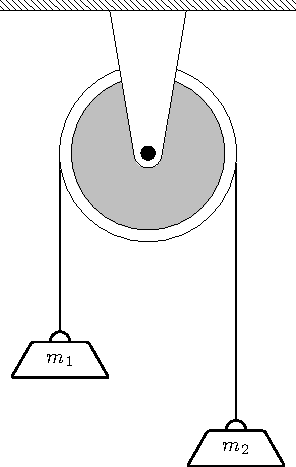
\includegraphics[width=0.3\textwidth]{./Images/atwood-machine.pdf}
	\caption{Diagrama de Maquina de Atwood Simple}
	\label{fig:atwood_machine}
\end{figure}

\subsection{Preguntas emergentes}
Después del planteamiento del sistema, el director Alfonso Leyva pregunta: \emph{¿Por qué es la cuerda inextensible y sin masa? ¿Cuales son las implicaciones de que la cuerda tuviese masa?} Si la cuerda no fuese inextensible se comportaría como un tipo de resorte y aparecería una fuerza y coeficiente adicional. Mientras que la masa supone la necesidad de una ecuación adicional para el sistema, pasando de tener 2 a 3 cuerpos.

\subsection{Ecuaciones de movimiento del sistema}
Por la construcción del sistema se tienen las siguientes condiciones de ligadura:

\begin{equation}
	\begin{cases}
		\begin{cases}
			x_1 = 0 &\implies f_1^{(h)} = x_1 = 0 \\
			z_1 = 0 &\implies f_2^{(h)} = z_1 = 0 \\
		\end{cases} & \text{, fijan el movimiento de } m_1 \\
		\begin{cases}
			x_2 = 0 &\implies f_3^{(h)} = x_2 = 0 \\
			z_2 = 0 &\implies f_4^{(h)} = z_2 = 0 \\
		\end{cases} & \text{, fijan el movimiento de } m_2 \\
		y_1 + y_2 = l  \implies f_5^{(h)} = y_1 + y_2 - l = 0  & \text{, acopla el movimiento de $m_1$ y $m_2$}
	\end{cases}
\end{equation}

Donde $l$ es la longitud de la cuerda sin contar la parte que gira sobre la correa, este termino se podría agregar sumando $\pi R$, $R$ siendo el radio de la polea, pero al final es una constante, y la solución no se vera afectada de tan grande forma.

Una vez más, usando la \Cref{eq:minim_coordinates} se obtiene que el numero mínimo de coordenadas generalizadas para dos cuerpos con 5 ligaduras es:

\begin{gather}
	s = 3(2) - 5 \\
	\therefore s = 1
\end{gather}

La energía cinética y la potencial están dadas por:

\begin{align}
	T &= \frac{1}{2} \left(m_1 \dot{y}_1^2 + m_2 \dot{y}_2^2 \right) \\
	V &= -g \left(m_1 y_1 + m_2 y_2 \right)
\end{align}

Y el Lagrangiano es:

\begin{equation}
	\mathcal{L} = \frac{1}{2} \left(m_1 \dot{y}_1^2 + m_2 \dot{y}_2^2 \right) + g \left(m_1 y_1 + m_2 y_2 \right)
\end{equation}

Sin embargo, el numero mínimo de coordenadas es 1, por ello se puede reemplazar $y_2$ en función de $y_1$ usando la ligadura $f_5^{(h)}$. Obteniendo:

\begin{equation}
	\mathcal{L} = \frac{1}{2} \left(m_1 + m_2 \right) \dot{y}_1^2 + \left(m_1 - m_2 \right)g y_1 + m_2 gl
\end{equation}

Al tener el lagrangiano, se aplica la ecuación de Euler-Lagrange para obtener las ecuaciones de movimiento del sistema

\begin{equation}
	\ddot{y}_1 - g\frac{\left(m_1 - m_2 \right)}{\left(m_1 + m_2\right)} = 0
\end{equation}

Pero al tener $\ddot{y}_1 = -\ddot{y_2}$

\begin{equation}
	\ddot{y}_{1,2} = \pm g \frac{\left(m_1 - m_2 \right)}{\left(m_1 + m_2\right)}
\end{equation}

Donde:

\begin{itemize}
	\item Si $m_1 = m_2 \implies \ddot{y}_{1,2} = 0$
	\item Si $m_1 > m_2 \implies \ddot{y}_1 > 0 \quad \land \quad \ddot{y}_2 < 0$
	\item Si $m_1 < m_2 \implies \ddot{y}_1 < 0 \quad \land \quad  \ddot{y}_2 > 0$
\end{itemize}

lo cual esta en acuerdo con lo establecido al plantear el problema.

\section{Profundización en el Concepto de Ligadura}
\begin{definition}[Ligadura]
	Las \emph{ligaduras} son funciones que establecen una relación entre coordenadas generalizadas.
\end{definition}

Hay dos tipos generales de ligaduras:

\begin{itemize}
	\item \textbf{Estructurales o de Construcción:} Son dadas por como se construye el sistema.
	\item \textbf{De Activación:} Entregan información de la evolución del sistema y dependen de como se ponga el sistema a funcionar.
\end{itemize}

Las ligaduras se pueden tomar como fuerzas de tipo $f(r_i, \dot{r}_i, t)$ y por el método me multiplicadores de Lagrange pueden ser obtenidas.

Adicionalmente se tienen las ecuaciones de ligadura y su clasificación:

\begin{itemize}
	\item \textbf{Unilaterales} La relación entre variables no puede ser expresada por medio de una igualdad i.e. $f \ne f(r_i, \dot{r}_i, t)$.
	\item \textbf{Bilateral} Pueden ser expresadas por medio de igualdades, correspondiendo a la fase activa de una ligadura unilateral. Estas se pueden dividir en:
		\begin{itemize}
			\item Cinemáticas: $f = f(r_i, \dot{r}_i, t)$.
			\item Geométricas: $f = f(r_i, t)$.
			\item Estacionarias: $f = f(r_i)$.
		\end{itemize}
\end{itemize}

\subsection{Clasificación de Sistemas Físicos}
Según las ligaduras que posea un sistema puede ser clasificado de las siguientes formas

\begin{itemize}
	\item \textbf{Holónomo:} Si todas las ligaduras son geométricas o cinemáticas integrables i.e. $\forall f, \, f = f(r_i, t) \quad \lor \quad \forall f = f(r_i, \dot{r}_i, t) \; \exists \; \int f$.
		\begin{itemize}
			\item Esclerónomo: Si todas las ligaduras son estacionarias i.e. $\forall f, \; f = f(r_i)$.
			\item Reónomo: Si alguna de las ligaduras depende explícitamente del tiempo e.g. $f = f(r_i, t)$.
		\end{itemize}
	\item \textbf{No Holónomo:} Si alguna de sus ligaduras es cinemática no integrable i.e. $\exists f = f(r_i, \dot{r}_i, t) \; : \; \nexists \int f$.
\end{itemize}

Los dos sistemas tratados fueron del tipo \emph{holónomo esclerónomo}, por ello surgió la pregunta \emph{¿Cual seria un ejemple de un sistema no holónomo?} Se da como ejemplo un disco que rueda sobre un plano sin deslizarse.

%TODO Add rolling disk
\begin{figure}[htbp!]
	\caption{Disco Rodando Sobre un Plano sin Deslizamiento}
	\label{fig:disk_rolling}
\end{figure}

Para ese sistema descrito por la \Cref{fig:disk_rolling}, pose las siguientes ligaduras:

\begin{equation}
	\begin{cases}
		\dot{x}\cos{\varphi} + \dot{y}\sin{\varphi} &= R\dot{\theta} \\
		\dot{x}\sin{\varphi} - \dot{y}\cos{\varphi} &= 0
	\end{cases}
\end{equation}

Expresando las ligaduras de forma diferencial:

\begin{align}
	\cos{\varphi} \, dx + \sin{\varphi} \, dy &= R d\theta \label{eq:dexact_theta}\\
	\sin{\varphi} \, dx - \cos{\varphi} \, dy &= 0 \label{eq:constrained_2}
\end{align}

De la \Cref{eq:dexact_theta} se obtiene

\begin{equation}
	\partial_x \theta = \frac{1}{R} \cos{\varphi} \quad \land \quad \partial_y \theta = \frac{1}{R} \sin{\varphi}
\end{equation}

y reemplazando en \Cref{eq:constrained_2} se obtiene

\begin{equation}
	\partial_y \theta \, dx = \partial_x \theta \, dy \quad \iff \quad x = y
\end{equation}

Esto muestra que la ligadura es integrable solo si el disco se mueve en la linea recta dada por $x = y$, del resto no es integrable y el sistema seria no holónomo.

\section{Aplicación}
Finaliza la exposición y el director Alfonso Leyva propone un problema para aplicar lo expuesto.

El problema consiste en un pingüino sobre un iglu de forma esférica, el cual se desliza sobre el mismo hasta caer al suelo. Se busca encontrar el angulo critico con respecto al centro del iglu en el cual el pingüino deja de estar en contacto con el iglu y procede a seguir en caída libre. La \Cref{fig:iglu} muestra un diagrama del problema.

%TODO Add Iglu figure

\begin{figure}[htbp!]
	\caption{Diagrama del Sistema}
	\label{fig:iglu}
\end{figure}

Debido a la naturaleza del sistema, se utilizan las coordenadas polares donde la energía cinética y potencial están dadas por:

\begin{align}
	T &= \frac{1}{2} m \left(\dot{r}^2 + \dot{r}^2 \dot{\theta}^2 \right) \\
	V &= -mgr\cos{\theta}
\end{align}

El lagrangiano resultando en:

\begin{equation}
	\mathcal{L} = \frac{1}{2}m \left(\dot{r}^2 + r^2\dot{\theta}^2 \right) - mgr\cos{\theta}
\end{equation}

La ligadura de este sistema es $f = r - R$, es del tipo de activación ya que representa si la fuerza normal esta actuando, ya que después del angulo critico no hay contacto con el iglu. Debido a esto, toca utilizar la ecuacion de Euler-Lagrange pero igualado a una fuerza generalizada i.e.

\begin{equation}
	\frac{d}{dt}\left(\partial_{\dot{q}} \mathcal{L}\right) - \partial_q \mathcal{L} = \lambda \partial_{q}f
\end{equation}

donde $\lambda$ representa un parámetro de ajuste o ``\emph{fine tuning}''.

Aplicando esta ultima ecuación se obtiene

\begin{align}
	m \left(\ddot{r} - r \dot{\theta}^2 + g\cos{\theta}\right) &= \lambda \\
	2r\dot{r}\dot{\theta} + r^2\ddot{\theta} - gr\sin{\theta} &= 0
\end{align}

Debido a la ligadura, $r = R \implies r^{(n)} = 0$ las ecuaciones se simplifican ha:

\begin{align}
	-mR\dot{\theta}^{2} + mg\cos{\theta} &= \lambda \label{eq:r_equation}\\
	R^2 \ddot{\theta} - gR\sin{\theta} &= 0 \label{eq:critical_theta}
\end{align}

Usando $\ddot{\theta} = \dot{\theta}\frac{d \theta}{d\theta}$, e integrando la \Cref{eq:critical_theta} se obtiene

\begin{equation}
	\dot{\theta} |_{\theta_c} = \frac{2}{R} g\left(1 - \cos{\theta_c} \right)
\end{equation}

Reemplazando en \Cref{eq:r_equation} y tomando las condiciones $\lambda = 0 \implies r = R \; \theta = \theta_c$. Se obtiene la expresión del angulo critico igual a:

\begin{equation}
	\cos{\theta_c} = \frac{2}{3}
\end{equation}

A partir de aplicar estas condiciones surge la pregunta \emph{¿Por qué se toma $\dot{r} = 0$ si en ese punto la velocidad no necesariamente es 0 y el movimiento sigue?} La razón radica en que el planteamiento va hasta el punto que se detiene el contacto, no se pretende describir lo que sucede después.

\end{document}
